\Large\textbf{\textcolor{blue}{3.}}
Evalúa el siguiente código en el lenguaje de programación \code{Racket}. Explica su resultado
y da la continuación asociada a evaluar, usando la notación $\lambda\uparrow$
\begin{lstlisting}
>(define c #f)
>(+ 1 (+ 2 (+ 3 (+ (let/cc k ( set! c k) 4) 5))))
>(c 10)
\end{lstlisting}

Se anexa captura de pantalla, sobre el resultado arrojado en \code{Racket}.
%%%%%%%     Imagen
\begin{center}
    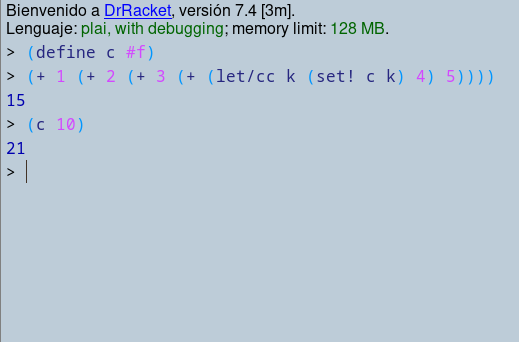
\includegraphics[scale=0.5]{Racket.png}
    \end{center}
%%%%%%%
Se evualúa de la siguiente forma:
\begin{itemize}
\item  Notación $\lambda\uparrow$ (\code{Racket}).\\
\code{(+ 1 (+ 2 (+ 3 (+ (let/cc k ( set! c k) 4) 5))))\\
(+ 1 (+ 2 (+ 3 (+ ($\lambda\uparrow$ (v) (v (+ 1 (+ 2 (+ 3 (+ 4 v )) 5))))))))\\
(+ 1 (+ 2 (+ 3 (+ ($\lambda\uparrow$ (v) (v (+ 1 (+ 2 (+ 3 (+ 4 5 ))))))))))\\
(v (+ 1 (+ 2 (+ 3 (+ 4 5)))))\\
(v 15) = 15
}\\

Se obtiene $15$ por que no se le pasa a la continuación el valor de $(c\;10)$
(con un argumento), por lo que este hace que \code{Racket} no lo considere para la
evaluación, haciendo que \code{Racket} solo tome la ''continuación actual'', entonces
la continuación de $c$ (en un inicio almacenando $\#f$) ahora contendrá a $4$.
\item  Notación $\lambda\uparrow$ (Se pasa (c 10)).\\
\code{(+ 1 (+ 2 (+ 3 (+ (let/cc k ( set! c k) 4) 5))))\\
(+ 1 (+ 2 (+ 3 (+ ($\lambda\uparrow$ (v) (v (+ 1 (+ 2 (+ 3 (+ 10 v )) 5))(c 10)))))))\\
(+ 1 (+ 2 (+ 3 (+ ($\lambda\uparrow$ (v) (v (+ 1 (+ 2 (+ 3 (+ 10 5 ))))))))))\\
(v (+ 1 (+ 2 (+ 3 (+ 10 5)))))\\
(v 21) = 21
}\\

Se obtiene $21$ por que se le pasa a la continuación el valor de $(c 10)$
(con un argumento), por lo que este hace que \code{Racket} lo considere para la evaluación de la continuación.
\end{itemize}
